\section{Funções compostas}

\begin{frame}[allowframebreaks]{Funções compostas}

\begin{itemize}
    \item Suponha que alguns valores de uma função $f$ estejam no domínio de uma função $g$. Pode-se então combinar $f$ e $g$ para formar uma nova função de $x$ e cujos valores são os números $g(f(x))$ (lê-se "$g$ de $f$ de $x$").

    \item Essa função, $g(f(x))$, é a composta de $g$ e $f$, tendo como notação $g \circ f$.

    \begin{figure}
        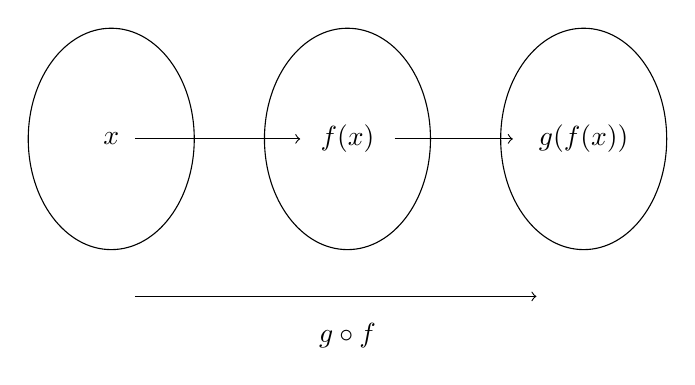
\begin{tikzpicture}
            \draw (0,0) ellipse (30pt and 40pt);
            \draw (3,0) ellipse (30pt and 40pt);
            \draw (6,0) ellipse (30pt and 40pt);

            \draw node at (0, 0) {$x$};
            \draw node at (3, 0) {$f(x)$};
            \draw node at (6, 0) {$g(f(x))$};

            \draw [->] (0 + 0.3, 0) -- (3 - 0.6, 0);
            \draw [->] (3 + 0.6, 0) -- (6 - 0.9, 0);

            \draw node at (3, -2.5) {$g \circ f$};
            \draw [->] (0 + 0.3, -2) -- (6 - 0.6, -2);
        \end{tikzpicture}
    \caption{Diagrama de composição das funções $g$ e $f$}
    \end{figure}

    \skipframe

    \item A função composta $g \circ f$ só está definida quando o contradomínio de $f$ é igual ao domínio de $g$. 
    
    \item Em geral, $g \circ f \neq f \circ g$.

    \item Pode acontecer que uma das funções $g \circ f$ ou $f \circ g$ não esteja definida.

    \skipframe

    \begin{ex}[Vendo uma função como uma composição]
        A função $y = \sqrt{1 - x^2}$ é a composição da função $g(x) = 1 - x^2$ com a função $f(x) = \sqrt{x}$. Ela pode ser pensada calculando-se primeiro $1 - x^2$ e depois tornando a raiz quadrada do resultado. Note que $1 - x^2$ não pode ser negativa. O domínio da composição é $[-1, 1]$.
    \end{ex}

    \skipframe

    \begin{ex}[Encontrando uma fórmula para a função composta]
        \emph{Dado $g(x) = x^2$ e $f(x) = x - 7$. Qual o valor de $f(g(2))$?} 

        \vspace{0.5cm}

        \textbf{R:} Para encontrar $f(g(x))$, substitui-se $x$ na fórmula $f(x) = x - 7$ pela expressão dada para $g(x)$: $f(g(x)) = g(x) - 7 = x^2 - 7 \Rightarrow f(g(2)) = 2^2 - 7 = -3$
        
    \end{ex}

    
\end{itemize}
    
\end{frame}